%%%%%%%%%%%%%%%%%%%%%%%%%%%%%%%%%%%%%%%%%%%%%%%%%%%%%%%%%%%%%%%%%%%%%%%%%%%%%%%%
% Template for USENIX papers.
%
% History:
%
% - TEMPLATE for Usenix papers, specifically to meet requirements of
%   USENIX '05. originally a template for producing IEEE-format
%   articles using LaTeX. written by Matthew Ward, CS Department,
%   Worcester Polytechnic Institute. adapted by David Beazley for his
%   excellent SWIG paper in Proceedings, Tcl 96. turned into a
%   smartass generic template by De Clarke, with thanks to both the
%   above pioneers. Use at your own risk. Complaints to /dev/null.
%   Make it two column with no page numbering, default is 10 point.
%
% - Munged by Fred Douglis <douglis@research.att.com> 10/97 to
%   separate the .sty file from the LaTeX source template, so that
%   people can more easily include the .sty file into an existing
%   document. Also changed to more closely follow the style guidelines
%   as represented by the Word sample file.
%
% - Note that since 2010, USENIX does not require endnotes. If you
%   want foot of page notes, don't include the endnotes package in the
%   usepackage command, below.
% - This version uses the latex2e styles, not the very ancient 2.09
%   stuff.
%
% - Updated July 2018: Text block size changed from 6.5" to 7"
%
% - Updated Dec 2018 for ATC'19:
%
%   * Revised text to pass HotCRP's auto-formatting check, with
%     hotcrp.settings.submission_form.body_font_size=10pt, and
%     hotcrp.settings.submission_form.line_height=12pt
%
%   * Switched from \endnote-s to \footnote-s to match Usenix's policy.
%
%   * \section* => \begin{abstract} ... \end{abstract}
%
%   * Make template self-contained in terms of bibtex entires, to allow
%     this file to be compiled. (And changing refs style to 'plain'.)
%
%   * Make template self-contained in terms of figures, to
%     allow this file to be compiled. 
%
%   * Added packages for hyperref, embedding fonts, and improving
%     appearance.
%   
%   * Removed outdated text.
%
%%%%%%%%%%%%%%%%%%%%%%%%%%%%%%%%%%%%%%%%%%%%%%%%%%%%%%%%%%%%%%%%%%%%%%%%%%%%%%%%

\documentclass[letterpaper,twocolumn,10pt]{article}
\usepackage{usenix2019_v3}
\usepackage{fontawesome}

% to be able to draw some self-contained figs
\usepackage{tikz}
\usepackage{amsmath}

\usepackage{spverbatim}

% inlined bib file
\usepackage{filecontents}
\usepackage[justification=centering]{caption}
%-------------------------------------------------------------------------------
\begin{filecontents}{\jobname.bib}
%-------------------------------------------------------------------------------
@Book{arpachiDusseau18:osbook,
  author =       {Arpaci-Dusseau, Remzi H. and Arpaci-Dusseau Andrea C.},
  title =        {Operating Systems: Three Easy Pieces},
  publisher =    {Arpaci-Dusseau Books, LLC},
  year =         2015,
  edition =      {1.00},
  note =         {\url{http://pages.cs.wisc.edu/~remzi/OSTEP/}}
}
@InProceedings{waldspurger02,
  author =       {Waldspurger, Carl A.},
  title =        {Memory resource management in {VMware ESX} server},
  booktitle =    {USENIX Symposium on Operating System Design and
                  Implementation (OSDI)},
  year =         2002,
  pages =        {181--194},
  note =         {\url{https://www.usenix.org/legacy/event/osdi02/tech/waldspurger/waldspurger.pdf}}}
\end{filecontents}

%-------------------------------------------------------------------------------
\begin{document}
%-------------------------------------------------------------------------------

%don't want date printed
\date{}

% make title bold and 14 pt font (Latex default is non-bold, 16 pt)
\title{\Large \bf Team A\\ \faicon{github} \href{https://github.com/danbachar/swiss-knife/tree/master/task1}{Task 1}}

%for single author (just remove % characters)
\author{
{\rm Dan Bachar}
\and
{\rm Yichao Zhu}
\and
{\rm Georgiy Nefedov}
% copy the following lines to add more authors
% \and
% {\rm Name}\\
%Name Institution
} % end author

\maketitle



%-------------------------------------------------------------------------------
\section{Basic Task}
%-------------------------------------------------------------------------------

\subsection{Description}

The essence of the first task is to master creating reproducible experiments using containers. In particular, this includes setting up several containers to host a WordPress blog, importing dummy data, setting up a Rest authentication plugin, running multiple HTTP benchmarks, and finding bottlenecks with full-system profiling. 

\subsection{Setup}

We decided to use the Docker container engine to make make our results reproducible for others. In the \texttt{docker-compose.yml} file we defined a MySQL database from the \texttt{mysql:5.7} image, a WordPress blog from the \texttt{wordpress:php7.3-fpm-alpine} image and a nginx web application from the \texttt{nginx:alpine} image.
For API authentication we installed the miniOrange API Authentication plugin and configured Basic Auth.

The light-weighted alpine-based images of \texttt{nginx} and \texttt{wordpress} only occupy 22.9MB and 264MB respectively. In order to persist the data and configuration files, we specify volumes on each container. The container-internal \texttt{nginx} port is mapped to the host port 8080, and it serves as a reverse proxy to the \texttt{wordpress} container whose port is 9000. The web server \texttt{php-fpm} will get requests from \texttt{nginx}, spawn working sub-processes, and interpret the Wordpress php scripts. The \texttt{mysql} database is working at port 3306.



\section{Benchmarking}

We benchmarked the request throughput of our WordPress blog setup by performing \texttt{GET} requests for retrieving the home page, and \texttt{POST} requests for adding a new page to the blog. To do this we tried out many different http benchmarking utilities. Httperf  \href{https://github.com/httperf/httperf}{httperf} turned out to be the most suitable. With \texttt{httperf} we can easily generate heavy loads of 10000+ request per second. We also compared the results with another tool, \texttt{wrk}, and they were similar.\\
The exact command to reproduce the benchmarks and the results can be found \href{https://github.com/danbachar/swiss-knife/blob/master/task1/benchmark/README.md}{here}.


\subsection{Retrieve the home page}

% TODO: update throughput
Using \texttt{httperf} we retrieved the front page \texttt{http://ryan.dse.in.tum.de:8080/} 1000 times. For simplicity, the rate is set to 0, it means that the connection will be generated sequentially (a new connection is initiated as soon as the previous one completes) and got the throughput \texttt{264.2 req/s} or \texttt{3.8 ms/req} with request size \texttt{71 B}.

\subsection{Create a page using the Rest API}

Please install and activate the `miniOrange API Authentication plugin` in wordpress to reproduce this part. \\
Also with \texttt{httperf} we sent 1000 POST requests to \texttt{http://ryan.dse.in.tum.de:8080/wp-json/wp/v2/pages} with the contents from \href{https://github.com/danbachar/swiss-knife/blob/master/task1/benchmark/bench2_content}{this file} to create a new blog page. The content size is about 6kB.\\
The throughput was \texttt{5.3 req/s} or \texttt{190.0 ms/req} with request size \texttt{6968 B}, about 50 times less then the simple GET request.

\subsection{Profiling}
We use some full-system profiling tools \texttt{perf, bcc} to analyse the bottlenecks in the system and generate the Flamegraph at figure \ref{flamegraph} . It shows hot function of the process. We can analyse from the flamegraph that the php-fpm process takes much more cpu times than mysqld. And there are two peaks, and five hot kernel space functions of php-fpm, namely \texttt{\_\_sys\_sendto}, \texttt{filename\_lookup}, \texttt{do\_sys\_poll}, \texttt{\_\_sys\_recvfrom} and \texttt{vfs\_read}. These kernel-space functions undertake the responsibility of communication. And they do not occupy too much time slices. So we have little need to optimise them. Most of the time are consumed by the user-space function, even though we can not get their symbols, we should know they are doing tasks like scripts interpretation and process management, which may also not have much room for optimization. So we need to find other ways to extend the system performance instead of trying to change the source code.
The details of this part can be found \href{https://github.com/danbachar/swiss-knife/blob/master/task1/benchmark/optimization.md}{here}. 

\begin{figure}
\centering 
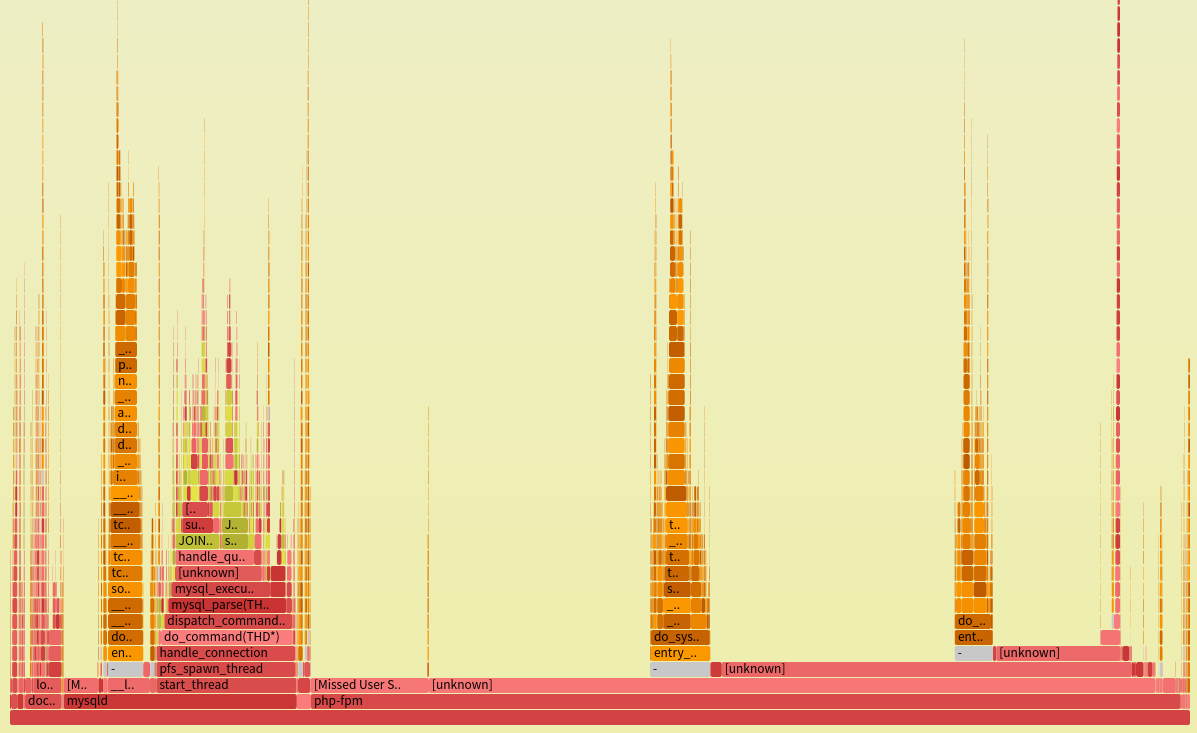
\includegraphics[width=0.4\textwidth]{task1/bccprofile.png}
\caption{Flamegraph} 
\label{flamegraph}
\end{figure}

\section{Exploration Task}

\subsection{Description}

The main objective of the exploration task is to optimise throughput and to demonstrate the effect of each optimization on throughput. It involves analysing system bottlenecks with the help of system profiling tools and trying to optimise them at various levels such as application server settings, caching, resource allocation, etc.

\subsection{Setup and Methodology}

We first increased the load on the system by using the http load testing method in the previous section with  and at the same time used the system monitor program(\texttt{top, sysstat, ss, docker stats}) to analyse the current usage of system resources such as cpu and memory, and analysed the hot functions in both user space and kernel space with the \texttt{bcc} system profiling tool. It was found that each \texttt{php-fpm} working process had enough CPU time to work, but the overall system performance was not fully utilized, so more child processes could still be forked to handle requests. At the same time, concurrent repeated requests would result in too many unnecessary database accesses, so the cache mechanism is used to increase the system.

\begin{figure}
\centering 
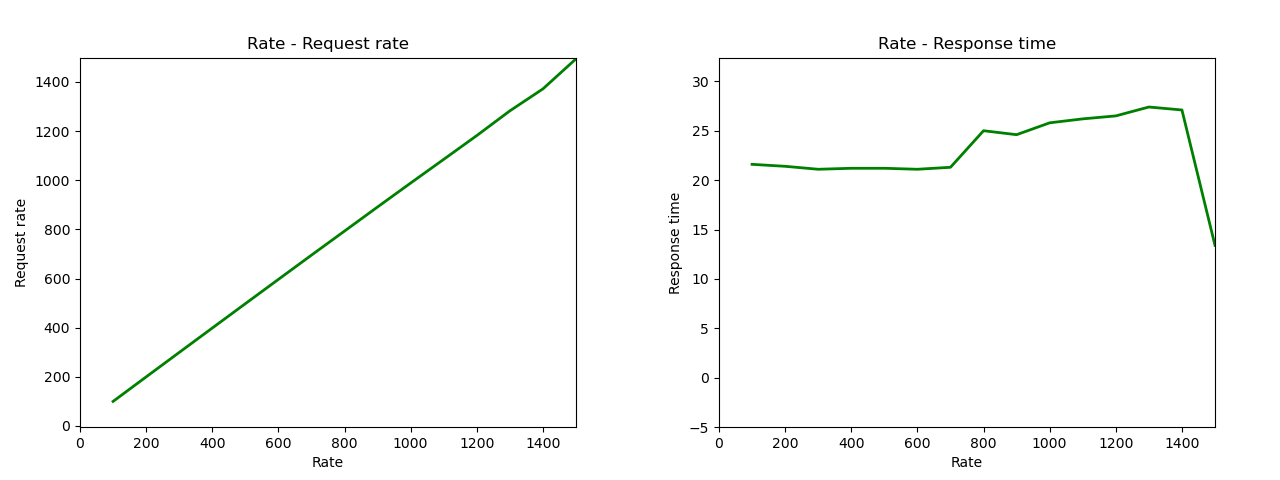
\includegraphics[width=0.45\textwidth]{task1/bm_25_mariadb.png}
\caption{25 php children with mariadb without cache reaches 1400 req/s} 
\label{bm_25_mariadb}
\end{figure}

\subsection{Result}

The original version of the nginx-php-mysql server had the throughput of \texttt{210 req/s} while requesting the front page with \texttt{GET}, after increasing the php-fpm's maximum amount of children working subprocesses to 25, it has reached a throughput of \texttt{1000+ req/s}.
Replacing MySQL with MariaDB has allowed us to go beyond to \texttt{1400+ req/s}, as shown in figure \ref{bm_25_mariadb}. With 70 php-fpm subprocesses, after activating a Wordpress cache plugin has allowed us to reach a cap of \texttt{35543 req/s} requests per second compared to the \texttt{5431.01 req/s} without cache. For details, please see the document \href{https://github.com/danbachar/swiss-knife/blob/master/task1/benchmark/optimization.md}{here}. 
\newline
The cache plugin has enabled a great improvement in our performance benchmarks because wordpress is a great candidate for caching. All wordpress pages are dynamic and are built by the requests with appropriate query and body parameters to a file called \texttt{index.php}. This file then builds the requested view for the user, and sends it back via the HTTP response. Since all of the benchmark requests are exactly the same, the plugin just has to create this file once, and statically serves this file to them, instead of going through the relatively expensive process of dynamically creating the requested view every time.
\newline
The Database replacement came to mind because it is extremely easy, as MariaDB is a drop-in replacement for MySQL. Here we created a SQL dump from the database inside the container, exported it to the host machine, replaced the databases and imported the dump in the new MariaDB database.
\newline
Changing \texttt{php-fpm}'s child creation policy from dynamic to static had also a noticeable effect since instead of waiting for the child processes to be dynamically created as demand arrives, the child processes are already initially available. 

%-------------------------------------------------------------------------------
\bibliographystyle{plain}
\begin{thebibliography}{99}  
\bibitem{ref1}https://docs.docker.com
\bibitem{ref2}https://www.brendangregg.com/flamegraphs.html
\bibitem{ref3}https://linux.die.net/man/1/httperf
\bibitem{ref4}https://medium.com/swlh/wordpress-deployment-with-nginx-php-fpm-and-mariadb-using-docker-compose-55f59e5c1a
\end{thebibliography}
%%%%%%%%%%%%%%%%%%%%%%%%%%%%%%%%%%%%%%%%%%%%%%%%%%%%%%%%%%%%%%%%%%%%%%%%%%%%%%%%
\end{document}
%%%%%%%%%%%%%%%%%%%%%%%%%%%%%%%%%%%%%%%%%%%%%%%%%%%%%%%%%%%%%%%%%%%%%%%%%%%%%%%%

%%  LocalWords:  endnotes includegraphics fread ptr nobj noindent
%%  LocalWords:  pdflatex acks